\chapter[Les m\`emes Internet, objets num\'eriques culturels]{Les m\`emes Internet, objets num\'eriques culturels}

Afin de mener \`a bien cette \'etude, nous avons choisi de nous int\'eresser \`a un objet num\'erique particulier : les \textit{m\`emes Internet}. Courts messages se propageant rapidement sur la Toile, les m\`emes proposent une illustration pertinente des discursivit\'es multiples qui prennent place dans les \'echanges en ligne. Plus que de simples blagues de potache, nous verrons ici comment ces constructions collectives \'eph\'em\`eres laissent parfois des traces symboliques qui structurent le milieu num\'erique qui les produit. Nous pr\'esenterons tout d{\textquoteright}abord la notion controvers\'ee de \textit{m\`eme, }d\'efinie d{\textquoteright}abord comme une unit\'e minimale de diffusion des cultures. Nous verrons ensuite comment ce concept teint\'e d{\textquoteright}un \'evolutionnisme peu convaincant flotte depuis sa cr\'eation en marge de la litt\'erature scientifique. En introduisant ensuite les \textit{m\`emes Internet}, nous observerons le fort regain de popularit\'e dont a b\'en\'efici\'e ce mot ces dix derni\`eres ann\'ees\textit{. }Nous envisagerons ensuite le r\^ole des m\`emes Internet - et \`a plus forte raison des technologies num\'eriques - en resituant leur \'etude dans la perspective historique plus large des questionnements sur la formation de m\'emoires collectives. En interrogeant notamment la notion de {\textquotedblleft}performativit\'e{\textquotedblright}, nous verrons comment les pratiques \textit{d{\textquoteright}\'enonciation }qui entourent les m\`emes Internet forment une pratique rh\'etorique et une activit\'e symbolique importante dans l{\textquoteright}actualisation et l{\textquoteright}\'echange de signes. Enfin, nous d\'etaillerons les processus discursifs entourant les m\`emes en proposant une cat\'egorisation selon l{\textquoteright}intention des \'enonc\'es, comme pr\'elude m\'ethodologique \`a notre d\'emonstration.

\section[Les m\`emes : d\'efinitions et histoire ]{Les m\`emes : d\'efinitions et histoire } 

Le dictionnaire d{\textquoteright}Oxford\footnote{ D{\textquoteright}apr\`es \textit{British \& Words English} publi\'e par Oxford University Press en 2014, \ \url{http://www.oxforddictionaries.com/definition/english/meme}, consult\'e le 24 F\'evrier 2014 \`a 21:50} donne deux d\'efinitions du mot \textit{m\`eme }: 

\begin{quote}
    \textit{Meme }(n.)

    \begin{enumerate}
        \item Un \'el\'ement d{\textquoteright}une culture ou syst\`eme de comportement pass\'e d{\textquoteright}un individu \`a un autre par imitation ou par d{\textquoteright}autres moyens non-g\'en\'etiques.
        \item Une image, vid\'eo, morceau de texte, etc., la plupart du temps de nature \ \ humoristique, qui est copi\'e(e) et propag\'e(e) rapidement par les utilisateurs \ \ d{\textquoteright}Internet, souvent apr\`es avoir \'et\'e modifi\'e(e).
    \end{enumerate}

\end{quote}

 Cette d\'efinition nous renseigne sur l{\textquoteright}usage de ce terme, en le d\'efinissant \`a la fois comme un \'el\'ement culturel transmissible et comme une forme particuli\`ere de contenus diffus\'e sur Internet. En nous appuyant sur son \'evolution dans la litt\'erature, nous allons tout d{\textquoteright}abord essayer de voir comment les deux versants de ce concept se sont historiquement articul\'es et \`a plus forte raison comment cette articulation peut nous servir pour comprendre les ph\'enom\`enes \`a l{\textquoteright}{\oe}uvre dans les r\'eseaux sociaux en Chine. 

\subsection[La m\'em\'etique : une \'ethologie culturelle teint\'e d{\textquoteright}\'evolutionnisme]{La m\'em\'etique : une \'ethologie culturelle teint\'e d{\textquoteright}\'evolutionnisme}

Le premier usage du concept de \textit{m\`eme} est souvent attribu\'e au biologiste Richard Dawkins dans son livre \textit{Le G\`ene \'ego\"iste }(1976). Dawkins s{\textquoteright}inspire des th\'eories \'evolutionnistes de l{\textquoteright}\'ethologie moderne pour proposer le \textit{m\`eme} comme un \'el\'ement mol\'eculaire de la culture qui permettrait sa transmission, semblable au g\`ene des individus biologiques. Consid\'er\'e comme une \textit{{\guillemotleft}~unit\'e d{\textquoteright}information culturelle qui peut \^etre copi\'ee, situ\'ee dans le cerveau~{\guillemotright}} \cite{Blackmore2001}, le m\`eme serait la fondation de pratiques culturelles qui \'evolueraient selon des variations de la s\'election naturelle. Repr\'esent\'e comme une {\guillemotleft}~\textit{unit\'e distincte de la pens\'ee {\guillemotright} }\cite{Dawkins1976}, le concept se fonde sur l{\textquoteright}analogie entre les processus de transmission culturelle et g\'en\'etique: \textit{{\textquotedblleft}Cultural transmission is analogous to genetic transmission in that, although basically conservative, it can give rise to a form of evolution{\textquotedblright} }(p.72)\textit{.} Cette approche \'ethologique de la culture consid\`ere donc le \textit{m\`eme} \`a la fois comme un \'el\'ement transmissible et un facteur de transmission dot\'e de la capacit\'e de se reproduire lui-m\^eme. \'El\'ement actif, le m\`eme serait donc un \textit{{\guillemotleft}~g\`ene \'ego\"iste {\guillemotright} }agissant de mani\`ere isol\'ee et distincte, sp\'ecificit\'e d{\textquoteright}une {\textquotedblleft}culture{\textquotedblright}. Plus encore, son~but unique serait sa propre p\'erennisation par sa propagation de cerveau en cerveau \cite{Blackmore1997}. Il agit donc comme un agent culturel poss\'edant une forme de volont\'e propre pour se propager. Souvent repr\'esent\'e gr\^ace \`a l{\textquoteright}image du virus, il donne l{\textquoteright}id\'ee d{\textquoteright}une propagation de la culture sous forme de contamination avec en arri\`ere-plan une lutte pour la survie et la f\'econdit\'e des id\'ees. Le m\`eme est un {\textquotedblleft}r\'eplicateur culturel{\textquotedblright}, une extension \`a part enti\`ere du vivant au-del\`a du biologique (Bloom, 2002). 

 Le qu\'eb\'ecois Fernand Dumont d\'efinit la culture comme cette \textit{{\guillemotleft}~maison o\`u l{\textquoteright}on habite ensemble~{\guillemotright} }\cite{Dumont1993}. N{\oe}ud dans une topologie sociale, le m\`eme pourrait donc \'egalement se pr\'esenter comme un point d{\textquoteright}entr\'ee, une porte entrouverte vers ce lieu o\`u d{\textquoteright}autres sont d\'ej\`a pass\'es et se trouvent encore. Le m\`eme devenu particule culturelle d\'efinit un seuil, ce lieu de passage si particulier qui \textit{{\guillemotleft}~fonde les espaces~{\guillemotright}} \cite{Bonnin2000} et invite ou interdit d{\textquoteright}entrer. Comme on enl\`eve ces chaussures au dojo et qu{\textquoteright}on sonne \`a la porte, les m\`emes sont peut-\^etre \`a envisager comme des rites de franchissement de seuils~culturels, pratiques de liaison du vivre-ensemble politique d{\textquoteright}Arendt (2001). Pour le g\`ene comme pour le m\`eme, il ne s{\textquoteright}agit pas de consid\'erer la fonction m\'ecanique d{\textquoteright}un {\textquotedblleft}r\'eplicateur{\textquotedblright} mais d{\textquoteright}observer l{\textquoteright}alt\'eration qui se d\'eroule lors de son actualisation pour en comprendre les limites et le r\^ole. La pr\'esence \textit{in potentia }d{\textquoteright}une unit\'e culturelle identique ne constitue pas n\'ecessairement une r\'ealit\'e in-formante pour des groupes sociaux ou des individus \cite{Lissack2004}. Les sciences de la communication ont largement \'etudi\'e depuis 50 ans les modalit\'es de transmission des informations. Les \'etudes sur la r\'eception notamment ont bien montr\'e qu{\textquoteright}il ne suffisait pas qu{\textquoteright}un message soit \'emis pour \^etre d\'ecod\'e et compris \cite{Katz1989}. D\'ej\`a avec Shannon et Weaver \cite{Jakobson1960}, l{\textquoteright}environnement exprim\'e par le concept de\textit{ bruit }vient alt\'erer largement les ph\'enom\`enes de transmission tout au long de leurs diffusions \cite{Chandler2008}. La m\'em\'etique, faute d{\textquoteright}\'etude de cas cons\'equentes et d{\textquoteright}applications th\'eoriques r\'eelles \cite{Jouxtel2014} a subi de nombreux revers conceptuels en s{\textquoteright}appuyant notamment sur l{\textquoteright}image peu cr\'edible d{\textquoteright}une transmission par r\'eplication quasi-m\'ecanique. Ignorant la dimension po\'etique des actes de transmission, cette vision m\'ecaniste issue d{\textquoteright}une rationalisation excessive refl\`ete pourtant les \'ecueils non-dits des approches scientifiques modernes. Thierry Bardini dans son livre \textit{Junkware }(2011) effectue une recherche extensive sur les discussions et consid\'erations qui entourent la partie non-codante de l{\textquoteright}ADN appel\'ee \textit{{\textquotedblleft}junk ADN{\textquotedblright}}. Analysant les discussions dans les publications scientifiques, il montre comment plus de 80\% des \'el\'ements structurant l{\textquoteright}ADN ont \'et\'e tr\`es t\^ot \'etiquet\'es comme {\textquotedblleft}bruit{\textquotedblright} puis {\textquotedblleft}junk{\textquotedblright}, car il \'etait impossible d{\textquoteright}identifier leur participation active au codage de prot\'eines. La m\'etaphore de ce \textit{{\textquotedblleft}junk non-codant{\textquotedblright} }si envahissant et la relative facilit\'e avec laquelle nous nous permettons de l{\textquoteright}ignorer d\'emontre la n\'ecessit\'e d{\textquoteright}une approche renouvel\'ee des ph\'enom\`enes complexes du vivant, et notamment de ceux de la transmission culturelle. D\'ej\`a clairement identifi\'ees dans les \'etudes en communication, les fonctions non-langagi\`eres notamment sont indispensables au bon d\'eroulement d{\textquoteright}un acte de langage. Ainsi si la suppression du bruit est souvent un pr\'ealable m\'ethodologique pour l{\textquoteright}\'etude scientifique, elle peut souvent fausser l{\textquoteright}approche exp\'erimentale et les conclusions th\'eoriques en refusant d{\textquoteright}admettre sa partialit\'e. L{\textquoteright}\'etude des m\`emes est encore largement en qu\^ete de reconnaissance scientifique et si la construction th\'eorique permettant d{\textquoteright}isoler des \'el\'ements culturels pour l{\textquoteright}\'etude parait int\'eressante, elle manque d{\textquoteright}une r\'eelle prise sur l{\textquoteright}observation et l{\textquoteright}analyse par l{\textquoteright}\'etude de cas notamment. La fermeture d\`es 2005 du \textit{Journal of Memetics}, parution de r\'ef\'erence de la discipline naissante est annonc\'e d\`es 2002 par un article de B. Edmonds \cite{Jouxtel2014}. Intitul\'e \textit{Three Challenges for the Survival of Memetics}, l{\textquoteright}article\textit{ }exhorte les chercheurs int\'eress\'es \`a produire ce que Edmonds juge comme le minimum indispensable pour gagner la reconnaissance des milieux scientifiques : \textit{{\textquotedblleft}a conclusive case-study; a theory for when memetic models are appropriate; and a simulation of the emergence of a memetic process.{\textquotedblright}} \cite{Edmonds2002}.  
En effet, il parait impossible d{\textquoteright}assoir scientifiquement la l\'egitim\'e du concept en se fondant uniquement sur une analogie de ph\'enom\`enes. Si le m\`eme a donc rat\'e sa cible dans le domaine scientifique, son acception plus r\'ecente sous la forme de contenus Internet a n\'eanmoins redonn\'e au concept une nouvelle vie dans la culture populaire. Dans le m\^eme temps, ce sens renouvel\'e a permis de d\'efinir pr\'ecis\'ement un domaine d{\textquoteright}application id\'eal et a permis l{\textquoteright}\'emergence de nouvelles \'etudes dont nous allons maintenant discuter. 

\subsection[ M\`emes Internet : d\'efinition, litt\'erature et exemples]{M\`emes Internet : d\'efinition, litt\'erature et exemples}

Contrairement au concept \'eth\'erique de m\`eme pr\'esent\'e dans la partie pr\'ec\'edente, la d\'efinition des \textit{m\`emes Internet }est de prime abord plus pragmatique. Il s{\textquoteright}agit de courts messages faits de texte, image, vid\'eo ou de son gagnant rapidement une forte popularit\'e sur Internet en \'etant partag\'es, comment\'es, r\'eappropri\'es puis transform\'es lors de leur diffusion. L{\textquoteright}utilisation du terme \textit{m\`eme Internet }pour d\'ecrire la diffusion de messages ne recouvre pas n\'ecessairement la dimension \'evolutive et culturelle du concept initial de Dawkins, mais garde l{\textquoteright}id\'ee g\'en\'erale d{\textquoteright}une circulation {\guillemotleft}~virale~{\guillemotright} d{\textquoteright}id\'ees parmi des groupes d{\textquoteright}individus\footnote{ \textit{"The meaning is not that far away from the original. It's anything that goes viral."}, Dawkins interview\'e par le magazine \textit{Wired} \url{http://www.wired.co.uk/news/archive/2013-06/20/richard-dawkins-memes}, consult\'e le 12/08/2013 \`a 7h53 GMT+8}. Le concept de m\`eme a tr\`es fortement gagn\'e en popularit\'e avec cette nouvelle acception. En 2012, il a notamment \'et\'e s\'electionn\'e parmi les 10 mots les plus marquants de l{\textquoteright}ann\'ee par le prestigieux dictionnaire am\'ericain Merriam-Webster. Ce choix a \'et\'e motiv\'e par la tr\`es forte popularit\'e sur Internet des images parodiques du politicien Mitt Romney apr\`es une bourde lors d{\textquoteright}une intervention t\'el\'evis\'ee aux Etats-Unis\footnote{ \textit{{\textquotedblleft}Words of the year 2012{\textquotedblright}}, Merriam-Webster \url{http://www.merriam-webster.com/info/2012words.htm} consult\'e le 25 F\'evrier 2014 \`a 19:01 GMT+1}. Ainsi, le mot \textit{m\`eme }dans une acception que nous prendrons ici soin de nommer \textit{m\`eme} \textit{Internet} est aujourd{\textquoteright}hui entr\'e dans le vocabulaire commun du Web. De nombreux sites sp\'ecialis\'es~(knowyourmeme.org, quickmeme.org, memefest.org, etc) ont vu le jour avec comme mission d{\textquoteright}archiver et de collecter ces pi\`eces de la culture web. Un des plus anciens m\`emes Internet est certainement l{\textquoteright}usage des \'emotic\^ones ou smileys, ces petites figures qui servent \`a exprimer des \'emotions dans le contexte d{\textquoteright}oralit\'e \'ecrite d{\textquoteright}Internet. Apparu dans les premiers jours du r\'eseau Internet, les \'emotic\^ones r\'epondent \`a un besoin d{\textquoteright}expression non-verbale dans la communication en ligne. Tr\`es simples \`a utiliser ou \`a modifier, les \textit{smileys }connaissent une popularit\'e rapide et se diversifient partout autour de la toile.  

\begin{figure}[h]
    \centering
    

    \begin{quote}
    19-Sep-82 11:44~~~ Scott E~ Fahlman~~~~~~~~~~~~ :-)

    From: Scott E~ Fahlman {\textless}Fahlman at Cmu-20c{\textgreater}

    ~
    
    I propose that the following character sequence for joke markers:

    ~~~~~~~ 

    :-)

    ~~~~~~~ 
    
    Read it sideways.~ Actually, it is probably more economical to mark things that are NOT jokes, given current trends.~ For this, use

    ~~~~~~~ 

    :-(

    \end{quote}
    \caption[la première mention du smiley par Scott Fahlman]{19 Septembre 1982 : la première mention du smiley par Scott Fahlman\protect\footnotemark, que l’on retrouve quelques jours plus tard sur les mailing lists les plus utilisées de l’époque : Arpanet\protect\footnotemark  et Usenet \protect\footnotemark}
    \label{fig:smiley-story}
\end{figure}

\footnotetext{D’après \url{http://www.cs.cmu.edu/~sef/Orig-Smiley.htm} archive consultée le 10 Août 2013 à 09 :15 GMT+8}
\footnotetext{Usenet mailing list \url{https://groups.google.com/forum/\#!msg/net.works/dzzAYYz9fYM/m6DZBY5ZpzUJ} sarchive consultée le 10 Août 2013 à 09 :25 GMT+8}
\footnotetext{Usenet mailing list \url{https://groups.google.com/forum/?hl=en\#!topic/net.news/tywzPO0NOtw} archive consultée le 10 Août 2013 à 09 :20 GMT+8}

L{\textquoteright}usage des \'emoticones s{\textquoteright}est aujourd{\textquoteright}hui largement r\'epandu, notamment chez les adolescents et jeunes adultes (D Derks, Bos, \& Von Grumbkow, 2007). Une r\'ecente \'etude a m\^eme montr\'e que les zones du cerveau stimul\'ees par la vue d{\textquoteright}\'emoticones \'etaient similaires \`a celles stimul\'ees lors de la vue d{\textquoteright}un visage, indiquant un ancrage symbolique profond de l{\textquoteright}usage de ces signes \cite{Churches2014}. Des \'emotic\^ones singuliers se sont \'egalement d\'evelopp\'es dans diff\'erentes langues pour exprimer des sentiments particuliers, propres au langage et \`a ses modes d{\textquoteright}expression. Le caract\`ere id\'eographique des langues chinoise et japonaise se pr\^ete particuli\`erement \`a ces jeux de dessin langagier. En chinois, le plus c\'el\`ebre exemple est sans doute le caract\`ere [56E7?] (jiong4) qui repr\'esente en langue ancienne une fen\^etre d{\textquoteright}o\`u provient la lumi\`ere et signifie {\guillemotleft}~lumineux~{\guillemotright}. Sa ressemblance avec une figure humaine (un \'emotic\^one) a fait renaitre ce caract\`ere d\'esuet qui signifie d\'esormais qu{\textquoteright}un utilisateur est agac\'e, embarrass\'e ou m\^eme choqu\'e. La conjonction {\textquotedbl}[56E7?]rz{\textquotedbl} a m\^eme \'et\'e invent\'e : [56E7?]repr\'esentant la t\^ete et \textit{rz} le corps agenouill\'e d{\textquoteright}une personne ; elle signifie l{\textquoteright}\'echec et le d\'esespoir. Cette particularit\'e des langues asiatiques donnent \`a l{\textquoteright}\'emotic\^one un r\^ole central dans la communication en ligne qui se traduit dans le design des interfaces. Les r\'eseaux sociaux chinois proposent tous par d\'efaut de multiples jeux d{\textquoteright}\'emotic\^ones disponibles pour l{\textquoteright}utilisateur qui communiquent ainsi tr\`es rapidement en images.  

\begin{figure}[h]
    \centering
    
\includegraphics[width=4.1669in,height=3.278in]{figures/chap2/chapitre2-img1.png}
    \caption[Un jeu d{\textquoteright}\'emotic\^ones de Weibo]{Un jeu d{\textquoteright}\'emotic\^ones sur \url{weibo.com} -- Consult\'e le 10 Aout 2013 \`a 10:00 GMT+8}
    \label{fig:emoticons-weibo}
\end{figure}


L{\textquoteright}exemple de l{\textquoteright}\'emoticone illustre donc la mani\`ere dont un \'el\'ement visuel et langagier vient constituer les pratiques en ligne, en relation proche avec la culture et le lieu qui l{\textquoteright}a fait na\^itre. 

Il est difficile de d\'efinir un m\`eme a priori par la nature de son contenu. N\'eanmoins, la structure de la diffusion d{\textquoteright}un message peut nous permettre de le d\'ecrire comme un m\`eme. Reproduisant en grande partie le cycle de vie classique d{\textquoteright}une information comme une rumeur ou une \textit{news, }les m\`emes poss\`edent des modes de diffusion en ligne assez d\'etermin\'es et pr\'evisibles. La plupart du temps, ils sont mis en circulation sur un petit nombre de sites sp\'ecialis\'es, avant d{\textquoteright}\^etre repris dans une premi\`ere phase par un assez petit nombre d{\textquoteright}utilisateurs qui se charge de les publier sur les r\'eseaux sociaux \cite{Bauckhage2011}. Les r\'eseaux sociaux agissent alors comme une chambre d{\textquoteright}\'echo, qui d\'etermine si le {\textquotedblleft}proto-m\`eme{\textquotedblright} encore en devenir deviendra m\`eme ou restera simple message isol\'e. Durant cette phase souvent nomm\'ee \textit{adoption,} le m\`eme entre en concurrence avec d{\textquoteright}autres informations sur les r\'eseaux sociaux o\`u les utilisateurs sont sans cesse \ sollicit\'es par d{\textquoteright}autres informations (Davenport \& Beck, 2001). Si l{\textquoteright}attention g\'en\'er\'ee par le m\`eme aupr\`es des utilisateurs atteint un pic suffisamment important, il faut environ 2h30 pour que les m\`emes rejoignent les pages des m\'edias plus traditionnels en commen\c{c}ant par les blogs, puis les sites d{\textquoteright}information (Leskovec, Backstrom, \& Kleinberg, 2009) . Ensuite, l{\textquoteright}attention envers le m\`eme d\'ecroit fortement et rapidement. La pr\'esence \'episodique de citations maintient l{\textquoteright}existence du m\`eme apparente dans des groupes d\'efinis \cite{Buchel2012}.

\begin{figure}[h]
    \centering
    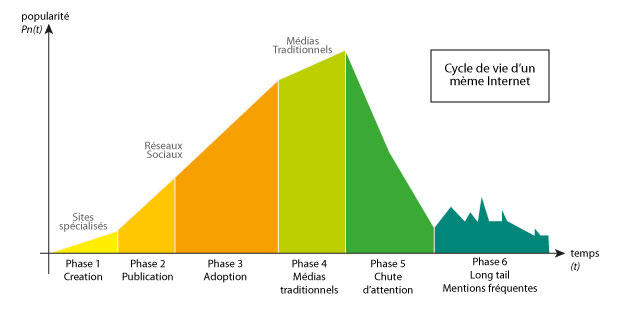
\includegraphics[width=6.2559in,height=3.1559in]{figures/chap2/chapitre2-img2.jpg}
    \caption[Cycle de vie d{\textquoteright}un m\`eme Internet]{Cycle de vie d{\textquoteright}un m\`eme Internet -Cl\'ement Renaud - 2013}
    \label{fig:meme-lifecycle}
\end{figure}

L{\textquoteright}\'evolution du volume de la diffusion permet donc de d\'efinir un m\`eme Internet. N\'eanmoins, il est impossible de donner une estimation du volume minimum pour devenir {\textquotedblleft}m\`eme{\textquotedblright} tant ce chiffre d\'epend de la population \'etudi\'ee : il existe des m\`emes \`a tr\`es forte diffusion comme le smiley ; d{\textquoteright}autres m\`emes se diffusent seulement au sein de groupes d{\textquoteright}individus restreints sans s{\textquoteright}\'etendre en-dehors. Ainsi, certains m\`emes peuvent avoir connu une diffusion tr\`es importante dans un groupe, mais rester absolument inconnu du reste de l{\textquoteright}Internet. Une \'etude de 2012 comparant la diffusion de nombreux m\`emes sur Twitter montre que les utilisateurs tendent \`a choisir les m\`emes selon la structure de leur r\'eseau social et le moment d{\textquoteright}exposition, produisant ainsi une grande h\'et\'erog\'en\'eit\'e des m\`emes dans le r\'eseau (Weng, Flammini, Vespignani, \& Menczer, 2012). Ainsi, il est hasardeux d{\textquoteright}essayer de d\'ecrire le concept de m\`eme par son contenu tant les sujets et les discussions varient. 

Quelques \'el\'ements d{\textquoteright}ordre grammaticaux peuvent n\'eanmoins \^etre observ\'es dans la forme que prennent les contenus, appel\'e parfois {\textquotedblleft}v\'ehicule{\textquotedblright} du m\`eme. Les m\`emes qui sont diffus\'es les plus largement sont compos\'es d{\textquoteright}images et de vid\'eo. L{\textquoteright}\'economie d{\textquoteright}attention tr\`es limit\'ee de l{\textquoteright}Internet et les modes de lecture sur \'ecran dans un contexte d{\textquoteright}abondance d{\textquoteright}information font que l{\textquoteright}on privil\'egie souvent les m\'edias visuels sur le texte \cite{Goldhaber2006}. Un autre \'el\'ement important est la facilit\'e avec laquelle un message peut \^etre appropri\'e par un utilisateur qui veut le modifier ou tout simplement le diffuser dans le r\'eseau. L{\textquoteright}existence des m\`emes est en effet largement conditionn\'ee par la possibilit\'e d{\textquoteright}une diffusion \`a moindre co\^ut et effort pour l{\textquoteright}utilisateur final, la plupart du temps non-r\'emun\'er\'e. Ici on voit \'emerger une structure visuelle caract\'eristique du m\`eme : une image accompagn\'ee d{\textquoteright}une l\'egende \'ecrite en caract\`eres blancs d\'etour\'es de noir, ou de caract\`eres blancs sur fond noir. L{\textquoteright}utilisation de haut contraste de couleur dans les typographies permet de faire apparaitre tr\`es efficacement des l\'egendes juxtapos\'ees \`a l{\textquoteright}image.


\begin{figure}[h]
    \centering
    
\includegraphics[width=3.6335in,height=2.9114in]{figures/chap2/chapitre2-img3.jpg}
    
\includegraphics[width=2.2559in,height=2.9449in]{figures/chap2/chapitre2-img4.jpg}
    \caption[Exemples de m\`emes internet]{Exemples de m\`emes Internet, d{\textquoteright}apr\`es \url{http://knowyourmeme.org}, consult\'e le 12/08/2013 \`a 10 :01 GMT+8}
    \label{fig:memes-examples}
\end{figure}


L{\textquoteright}usage d{\textquoteright}images l\'egend\'ees est une des formes les plus communes pour les m\`emes Internet, en particulier ceux de nature comique ou absurde. La mise en place de sites permettant de g\'en\'erer rapidement ce type d{\textquoteright}images l\'egend\'ees (memegenerator.com, mememachine.com, etc.) renforcent l{\textquoteright}unit\'e formelle des m\`emes sur l{\textquoteright}Internet, ou plut\^ot sur l{\textquoteright}Internet anglophone et francophone notamment. En effet, on constate que cette forme typique du m\`eme ne se retrouve pas sur l{\textquoteright}Internet chinois qui utilise plus volontiers des montages d{\textquoteright}images ou des jeux de mots, avec davantage de diversit\'e dans les formes que peuvent prendre les diff\'erents m\`emes.

\section[M\`eme, m\'emoire collective et culture]{M\`eme, m\'emoire collective et culture}
\subsection[La m\'emoire comme trace]{La m\'emoire comme trace}

Si le concept de m\`eme est souvent consid\'er\'e comme tr\`es r\'ecent, on peut n\'eanmoins le resituer facilement dans le vaste paysage des travaux sur la m\'emoire collective qui ont exist\'e depuis le XIX\`eme si\`ecle \cite{Laurent1999}. Max Stirner dans son livre \textit{The Ego and Its Own }(1844) \'enonce d\'ej\`a l{\textquoteright}id\'ee que les individus sont sujets \`a la circulation de concepts issus de souvenirs communs ou illusoires, comme notamment le nationalisme et la religion. Le logicien Bertrand Russell reprend par la suite dans son livre \textit{The Analysis of Mind }(1921) les travaux sur la m\'emoire et l{\textquoteright}\'evolution sociale du physiologiste allemand Richard Semon (1904). Utilisant le concept central de \textit{mneme} (du grec 
%\textit{$\mu \nu \text{\textgreek{'h}}\mu \eta $ }  
mneme, m\'emoire), Semon travaille sur l{\textquoteright}id\'ee de \textit{{\textquotedblleft}traces mn\'esiques{\textquotedblright} }laiss\'ees par les diverses exp\'eriences au niveau cellulaire comme au niveau de l{\textquoteright}organisme tout entier. La psychanalyse a \'egalement cherch\'e \`a saisir cette distance impalpable entre exp\'erience et organisme en interrogeant les marques laiss\'ees par les souvenirs. Pour Freud comme pour Semon, {\textquotedblleft}l{\textquoteright}appareil psychique{\textquotedblright} de la m\'emoire se constitue sous la forme de {\textquotedblleft}traces{\textquotedblright}, qu{\textquoteright}il se refuse n\'eanmoins \`a localiser dans des zones sp\'ecifiques du cerveau. Lacan apr\`es lui sugg\`erera que la perception et la m\'emoire des exp\'eriences se structurent dans le langage lui-m\^eme, seul outil de connaissance du monde. Depuis les dix derni\`eres ann\'ees, plusieurs d\'ecouvertes dans le domaine de la neurologie viennent corroborer cette id\'ee que la m\'emoire existe sous forme de traces. Les travaux autour de la \textit{plasticit\'e neuronale }montrent notamment l{\textquoteright}existence de la m\'emoire sous la forme de connections, relations t\'enues ancr\'ees dans notre r\'eseau neuronal global (Magistretti \& Ansermet, 2012).  

\begin{tabular}{c|c|c|c}

  \hline
    Etapes constituantes de la mémoire & t=1  & t=2  & t=3 \\
  \hline
    Freud  & expérience  & perception  & Traces mnémiques et psychiques \\
  \hline
    Lacan & expérience(signifié)  &   perception(signifié)  &   Signifiant (traces structurées dans le langage) \\
  \hline
    Neurosciences &  expérience & Perception & Traces synaptiquesassemblages de neurones \\
    \hline
\end{tabular}

\textit{fig. Convergence entre la trace psychique et synaptique
(Magistretti \& Ansermet, 2012)}


Ces disciplines s{\textquoteright}int\'eressent majoritairement \`a l{\textquoteright}\'etude de la constitution d{\textquoteright}une m\'emoire individuelle, ne nous livrant que peu de cl\'es pour comprendre les \'el\'ements qui font qu{\textquoteright}une m\'emoire devient commune. Le pal\'eontologiste Leroi Gourhan propose dans son livre \textit{L{\textquoteright}homme et la Mati\`ere }de consid\'erer que les humains poss\`edent trois formes de m\'emoire : une m\'emoire individuelle sensible, stock\'ee dans les organes du corps ; une m\'emoire h\'erit\'ee g\'en\'etiquement, stock\'ee dans l{\textquoteright}ADN ; et une troisi\`eme forme de m\'emoire, transmise de g\'en\'erations en g\'en\'erations : la \textit{technologie}. Dans sa lecture de Leroi-Gourhan, Stiegler (1998b) explique comment \textit{l{\textquoteright}objet technologique} porte en lui les traces des exp\'erimentations, r\'eussites et \'echecs pass\'es, m\'emoire cumulative de temps et de soci\'et\'es pass\'ees, \`a la fois h\'erit\'ee et commune, transmissible par son usage.

\begin{tabular}{|l|c|r|}
    \hline
    Forme de mémorie   &  Contenu  & Stockage \\
    \hline
    génétique  &  Particularités héritées des ancêtres   &  DNA \\
    \hline
    épigénétique   &  Mémoire sensible de l’expérience personnelle   &  Organes, nerfs, cerveau \\
    \hline
    technologique  &  Pratiques de la vie quotidienne en société (usages) & Objets technologiques \\
\end{tabular}

Fig. Les trois formes de m\'emoire d{\textquoteright}apr\`es
Leroi-Gourhan et Stiegler

\subsection[Diffusion de m\`emes et structuration d{\textquoteright}une m\'emoire collective]{2.2.2. Diffusion de m\`emes et structuration d{\textquoteright}une m\'emoire collective}
La relation entre m\'emoire humaine et m\'emoire technologique est au centre de notre \'etude. La technologie a depuis toujours \'et\'e consid\'er\'e comme une m\'emoire ext\'erieure. Dans \textit{Ph\`edre, }Platon raconte l{\textquoteright}histoire du roi \'egyptien Thamous recevant en cadeau du dieu Thot l{\textquoteright}\'ecriture, le rem\`ede (\textit{pharmakon) }qui devait \textit{{\textquotedblleft}soulager la science et la m\'emoire{\textquotedblright} }(Platon, 274e). Le roi Thamous, effray\'e par cette nouvelle technologie de la m\'emoire qu{\textquoteright}est l{\textquoteright}\'ecriture se voit saisi de l{\textquoteright}angoisse d{\textquoteright}une perte de cette m\'emoire. Avec la fin de cette oralit\'e, la disparition de la m\'ethode active des antiques th\'e\^atres de la m\'emoire au profit d{\textquoteright}une m\'emoire technologique inerte et ext\'erieure \`a soi pourrait-t-elle sceller l{\textquoteright}av\`enement d{\textquoteright}une nouvelle b\^etise? Aujourd{\textquoteright}hui, l{\textquoteright}importance grandissante des bases de donn\'ees et de connaissances soul\`event encore une fois les m\^emes questions, toujours irr\'esolues. Nicolas Carr constate notamment que \textit{{\textquotedblleft}l{\textquoteright}Internet nous rend stupide{\textquotedblright}} et que son usage r\'ep\'et\'e entraine une baisse drastique de nos facult\'es de concentration \cite{Carr2010}. A l{\textquoteright}\`ere du Big Data et de l{\textquoteright}expansion sans fin de notre m\'emoire num\'erique, la constitution de nos bases de donn\'ees interroge notre construction d{\textquoteright}une m\'emoire collective. Les m\`emes Internet, d{\textquoteright}abord grav\'es dans les disques durs des serveurs, viennent \^etre actualis\'es par ceux qui les partagent, les commentent, jouent avec et se les approprient. L{\textquoteright}exemple de l{\textquoteright}Internet chinois nous montre la volatilit\'e de cette m\'emoire num\'erique, artefact historiographique d{\textquoteright}une culture soumise au bon-vouloir des administrateurs du r\'eseau. Le Manifeste de l{\textquoteright}Archiviste publi\'e par Yuk Hui (2014) s{\textquoteright}ouvre sur l{\textquoteright}angoissante interrogation deleuzienne :  \begin{quote}
Un nouvel archiviste est nomm\'e dans la ville. Mais est-il \`a proprement parler nomm\'e ?
N'est-ce pas sur ses propres instructions qu'il agit ? 
\cite{Deleuze1984}.
\end{quote}

L{\textquoteright}existence et l{\textquoteright}usage quotidien des bases de donn\'ees questionnent chaque jour l{\textquoteright}assujettissement des symboles de notre m\'emoire \`a l{\textquoteright}objet technologique, \`a la fois b\'equille, proth\`ese et maquillage postiche de notre d\'etestable devenir b\^ete. L{\textquoteright}\'etude des m\`emes Internet nous offre ici une fen\^etre pour porter notre regard sur ces objets dont le corps scell\'ee dans les profondeurs glac\'ees des \textit{data centers }nous parvient en dansant, d{\textquoteright}abord sur nos \'ecrans puis dans un coin de notre t\^ete. Avec l{\textquoteright}usage r\'ep\'et\'e des technologies et de l{\textquoteright}\'ecriture num\'erique, les fronti\`eres entre milieu num\'erique et m\'emoire collective s{\textquoteright}estompent pour laisser entrevoir un enchev\^etrement de silicium, d{\textquoteright}id\'ees et de chair, constitutifs de notre savoir moderne. 

Poursuivant l{\textquoteright}id\'ee d{\textquoteright}une arch\'eologie du pr\'esent introduite par Foucault, il s{\textquoteright}agit donc de documenter les processus par lesquels ces obscurs habitants des bases de donn\'ees viennent laisser leurs traces pour constituer des bribes de nos m\'emoires collectives. Maurice Halbwachs dans son vaste travail aborde les fa\c{c}ons dont l{\textquoteright}histoire structure l{\textquoteright}\^etre-ensemble des groupes humains. En disant que \textit{"l'histoire de notre vie fait partie de l'histoire en général"}\cite{Halbwachs1947}, il identifie une m\'emoire autobiographique (personnelle) et une m\'emoire historique (sociale). Les inqui\'etudes et consid\'erations autour de la {\textquotedblleft}vie priv\'ee{\textquotedblright} sur Internet illustrent les liens intimes entre ces deux m\'emoires aux fronti\`eres devenant aujourd{\textquoteright}hui chaque jour plus poreuses. L{\textquoteright}acte singulier et autobiographique devient sous l{\textquoteright}effet du r\'eseau un fait social, disponible \`a tout moment dans {\textquotedblleft}l{\textquoteright}historique{\textquotedblright} qui se d\'eroule sous le curseur. L{\textquoteright}oubli devient alors un commerce tr\`es pris\'e permettant de garantir la limite entre la m\'emoire autobiographique de la fin de soir\'ee de samedi dernier et la m\'emoire socialement acceptable du CV du chercheur d{\textquoteright}emploi. \`A l{\textquoteright}inverse, les photos du dernier voyage en Papouasie ou la pose avec une star de la t\'el\'e t\'emoignent fi\`erement d{\textquoteright}un lien m\'emoriel entre autobiographie et histoire commune. Les \textit{m\`emes} se propagent ainsi d{\textquoteright}individus en groupes pour former peu \`a peu des \'el\'ements de m\'emoire commune. Objets, chansons, histoires, l\'egendes, ic\^ones... leur diffusion autour de la toile se fait par diff\'erents proc\'ed\'es tenant autant de la copie que de l{\textquoteright}appropriation. 

Le site de questions/r\'eponses \textit{Quora.com} offre un regard int\'eressant sur cette question puisque nous y trouvons une question : \textit{{\guillemotleft}~What are some quintessential Indian memes ?~{\guillemotright}.} Les utilisateurs r\'epondent donc en ajoutant des exemples de m\`eme qui semblent appartenir dans leurs esprits \`a la {\textquotedblleft}quintessence des m\`emes indiens {\textquotedblright}. 

\begin{figure}[h]
    \centering
    
\includegraphics[width=1.6224in,height=1.6224in]{figures/chap2/chapitre2-img5.jpg}
    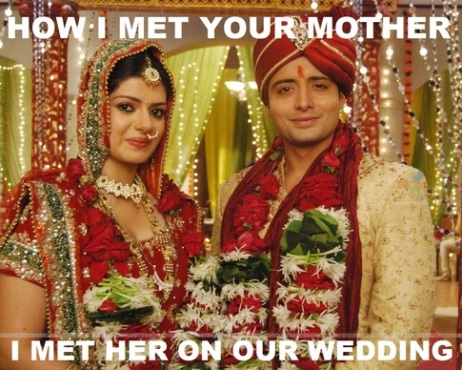
\includegraphics[width=2.0449in,height=1.6335in]{figures/chap2/chapitre2-img6.jpg}
    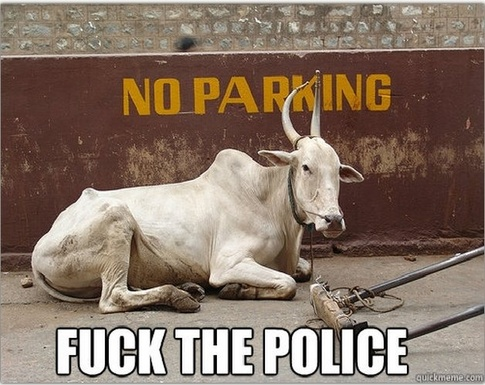
\includegraphics[width=2.078in,height=1.6449in]{figures/chap2/chapitre2-img7.jpg}
    \caption{Exemples de r\'eponses \`a la question \textit{"What are some quintessential Indian memes ?"} D'apr\`es \url{http://www.quora.com/India/What-are-some-quintessential-Indian-memes}, Consult\'e le 12/08/2013 \`a 0 :41 GMT+8 }
    \label{fig:quora-india}
\end{figure}


Avec plusieurs centaines d{\textquoteright}images post\'ees par des
utilisateurs majoritairement indiens\textsuperscript{7}, nous pouvons
constater plusieurs choses : 

\begin{itemize}
\item
\textbf{Langue}: à part trois réponses, la totalité des réponses sont en anglais. Cela peut s’expliquer par le fait que l’anglais est une langue de communication majoritaire en Inde, et également par le fait que le site Quora.com n’accepte habituellement que des réponses en anglais.
\item
\textbf{Forme}: à l’exception de quatre réponses, les mèmes revêtent tous la forme « classique » : photo retouchée et légendé par un texte en anglais aux lettres blanches sur fond ou détour noir.

\item
\textbf{Humour}: la plupart des réponses sont de nature comique.
\item
\textbf{Récurrence}: certaines images sont très récurrentes et si les légendes diffèrent, le sens reste le même.
\item
\textbf{Thématiques diverses}: de nombreux messages traitent de la vie de famille (parents, mariage), de loisirs (cricket), de la vie quotidienne (achats, école , etc.) et un peu de politique.
\end{itemize}

L{\textquoteright}image la plus cit\'ee repr\'esente la figure
d{\textquoteright}un p\`ere autoritaire :

\begin{figure}
    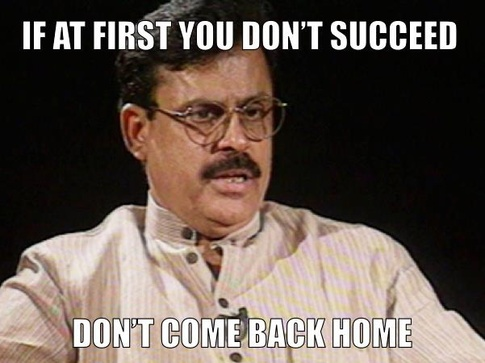
\includegraphics[width=2.0449in,height=1.5335in]{figures/chap2/chapitre2-img8.jpg}
    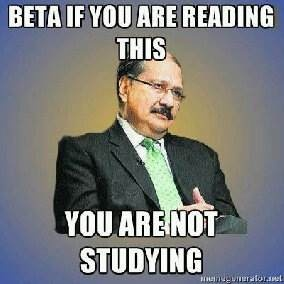
\includegraphics[width=1.5335in,height=1.5335in]{figures/chap2/chapitre2-img9.jpg}
    
\includegraphics[width=1.8224in,height=1.5449in]{figures/chap2/chapitre2-img10.jpg}
    \caption[\textit{"High Expectations Indian Father"} d'après Quora.com]{Exemples de m\`emes du \textit{p\`ere indien autoritaire}}
    \label{fig:severe-indian-dad}
\end{figure}



\'Etonnement, il existe un m\`eme plut\^ot similaire avec un p\`ere asiatique cette fois : 


\begin{figure}
    
\includegraphics[width=1.9335in,height=1.9224in]{figures/chap2/chapitre2-img11.png}
    
\includegraphics[width=1.9004in,height=1.8894in]{figures/chap2/chapitre2-img12.jpg}
    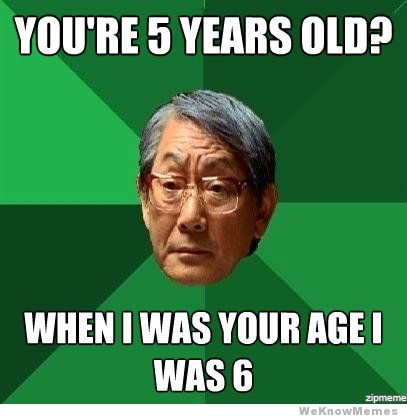
\includegraphics[width=1.8449in,height=1.9004in]{figures/chap2/chapitre2-img13.jpg}
    \caption[\textit{"High Expectations Asian Father"} d'après Quora.com]{Exemples du m\`eme \textit{"High Expectations Asian Father"} D{\textquoteright}apr\`es {\textquotedblleft}\textit{What are the funniest High Expectations Asian Father meme images?{\textquotedblright}} sur Quora.com \url{http://www.quora.com/Memes/What-are-the-funniest-High-Expectations-Asian-Father-meme-images}, Consult\'e le 12/08/2013 \`a 10:56}
    \label{fig:severe-chinese-dad}
\end{figure}

La d\'efinition des m\`emes faites par Blackmore ne correspond pas n\'ecessairement \`a ce que nous observons ici. L{\textquoteright}unit\'e formelle de l{\textquoteright}ensemble de ces m\`emes (image avec des caract\`eres blancs cercl\'es de noirs) propose une d\'efinition bien plus restreinte. N\'eanmoins, nous pouvons comprendre qu{\textquoteright}il s{\textquoteright}agit bien de la manifestation d{\textquoteright}une culture particuli\`ere. L{\textquoteright}image d{\textquoteright}une vache assise devant un sigle \textit{{\textquotedblleft}Fuck The Police{\textquotedblright} }serait en effet un absolu non-sens sans la r\'ef\'erence \`a l{\textquoteright}Inde o\`u les vaches sont sacr\'ees et jouissent de droits particuliers que m\^eme la police ne peut entraver. Ainsi, il existe bel et bien des pr\'e-requis pour comprendre ou actualiser un m\`eme. Les plus \'evidents sont :

\begin{itemize}
    \item \textbf{L’accès et l’usage de la bonne technologie}: Il est nécessaire pour un utilisateur de posséder et de savoir utiliser la technologie par laquelle le mème est diffusé.
    \item \textbf{La langue}: Le message possède une légende donc l’utilisateur doit pouvoir la lire et la comprendre.
    \item \textbf{Les implicites} : L’utilisateur doit posséder le socle de références communes et d’implicites qui sont impératifs pour pouvoir comprendre le message. 
\end{itemize}

Nous observons ici de tr\`es larges et vagues groupes ({\guillemotleft}~\textit{indiens}~{\guillemotright}, {\guillemotleft}~\textit{asiatiques}~{\guillemotright}{\dots}) sans pouvoir vraiment comprendre dans le d\'etail ce qui peut r\'eellement constituer des \'el\'ements communs. Les travaux sur la formation des {\textquotedblleft}communaut\'es{\textquotedblright} en ligne ont montr\'e comment la circulation des objets digitaux peut poss\'eder une fonction de catharsis pour des groupes plus r\'eduits \cite{Steyer2006}. N\'eanmoins, on voit bien qu{\textquoteright}ici l{\textquoteright}appartenance pr\'e-existe puisque le m\`eme n\'ecessite de nombreux pr\'e-requis pour le comprendre. Le langage et son expressivit\'e par l{\textquoteright}humour sont notamment des contraintes incompressibles pour l{\textquoteright}actualisation de ce m\`eme par un individu. N\'eanmoins nous pouvons voir dans ce cas particulier que le m\`eme participe \`a l{\textquoteright}affirmation de l{\textquoteright}existence du groupe, avec la figure redondante de caract\'eristiques communes du p\`ere, affirmant par la d\'erision une forme de paternit\'e commune aux membres de ce groupe. D{\textquoteright}autres m\`emes ne n\'ecessitent pas tant de r\'ef\'erences, ce qui contribue largement \`a leurs diffusions. La vid\'eo du clip musical \textit{Gangnam Style} du chanteur Psy a notamment atteint des records in\'egal\'es en termes de diffusion\footnote{ Premi\`ere vid\'eo \`a avoir officiellement d\'epass\'ee le milliard de vues sur Youtube. 1,733,769,243 vues, consult\'e le 13/08/2013 \`a 09 :35 GMT+8 \url{http://www.youtube.com/watch?v=9bZkp7q19f0}} gr\^ace \`a une tr\`es vaste campagne t\'el\'evisuelle et sur internet. La diminution des implicites et la standardisation de l{\textquoteright}\'ecriture utilis\'ee a sans doute contribu\'e la diffusion, avec un langage du corps quasi universel, le pas de danse. Formellement, il s{\textquoteright}agit d{\textquoteright}un vid\'eo clip tr\`es classique dont la structure et le montage sont largement familiers au public. Les attributs des personnages du clip sont \'egalement de grands classiques du vid\'eo clip commercial : voitures, belles filles et bijoux en or. La pr\'esence d{\textquoteright}un quartier sp\'ecifique de S\'eoul en Cor\'ee du Sud agit ici comme un attribut du contenu mais aucune des r\'ef\'erences ne n\'ecessite de pr\'ealable linguistique particulier. De plus, les myst\`eres de la musique et de la sc\'enographie agissent bien \'evidemment au del\`a de toute analyse formelle pour faire de ce hit un des m\`emes Internet les plus connus dans le monde. 
Les m\'em\'eticiens disposent classiquement de deux proc\'edes pour
analyser la diffusion des m\`emes: 

\begin{itemize}
\item
\textbf{La contamination~\newline
}Le m\`eme se d\'eplace \`a la mani\`ere d{\textquoteright}un virus, en contaminant les sujets les plus susceptibles de l{\textquoteright}\^etre lors d{\textquoteright}une phase d{\textquoteright}exposition. L{\textquoteright}exemple le plus classique pour ce mod\`ele est la diffusion des croyances religieuses
qui agirait par contagion \cite{Dennett2006}
\item
\textbf{La r\'eplication~\newline
L}es activit\'es culturelles humaines proc\`edent de l{\textquoteright}imitation, notamment au travers de phases cruciales d{\textquoteright}apprentissage. Ainsi, les m\`emes existent et se diffusent dans toutes activit\'es n\'ecessitant une imitation : \textit{{\textquotedblleft}} \textit{If we define memes as transmitted by imitation then whatever is passed on by this copying process is a meme.{\textquotedblright} }\cite{Blackmore2006}. 
\end{itemize}

Le mod\`ele \'epid\'emique de diffusion vient appuyer la vision \'ethologique du m\`eme. Adapt\'ee de la virologie, les {\guillemotleft}~sujets \`a risque~{\guillemotright} seraient plus \`a m\^eme d{\textquoteright}\^etre {\guillemotleft}~contamin\'es~{\guillemotright} par une {\guillemotleft}~exposition~{\guillemotright} suffisamment longue \`a tel ou tel m\`eme (Wang \& Wood, 2011). Blackmore d\'efinit n\'eanmoins trois phases indispensables pour reconna\^itre un m\`eme comme tel:  

\begin{quote}
Memes fulfill the role of replicator because they exhibit all three of the necessary conditions; that is, \textit{heredity} (the form and details of the behavior are copied), \textit{variation} (they are copied with errors, embellishments or other variations), and \textit{selection} (only some behaviors are
successfully copied).
(ibid.)
\end{quote}

Les trois aspects sont indissociables et forment selon Blackmore un {\textquotedblleft}\textit{v\'eritable processus \'evolutioniste{\textquotedblright} }(ibid.). La d\'efinition quasi tautologique du m\`eme ({\guillemotleft}~\textit{Whatever is passed on{\guillemotright}}) montre bien comment le m\`eme en tant que concept est consid\'er\'e chez Blackmore non pas comme un ph\'enom\`ene mais plut\^ot comme un objet en-soi. La d\'efinition du m\`eme en tant qu{\textquoteright}objet autonome se heurte d\`es l{\textquoteright}abord au risque de devenir un pur artefact de l{\textquoteright}observation, n{\textquoteright}existant que dans l{\textquoteright}esprit de l{\textquoteright}observant. Alors que Dawkins met en garde non sans humour que son livre \textit{The Selfish Gene} \textit{{\textquotedblleft}devrait \^etre lu presque comme s{\textquoteright}il \'etait de la science-fiction{\textquotedblright} }\cite{Dawkins1984}, la faiblesse des mod\`eles de diffusion des m\`emes vu comme un r\'eplicateur ou comme un virus ne recouvre que partiellement la r\'ealit\'e observ\'ee empiriquement pour les m\`emes Internet. Ainsi, l{\textquoteright}appartenance des individus \`a tel ou tel groupe pr\'e-existe au m\`eme. Dans son appropriation se joue davantage l{\textquoteright}expression d{\textquoteright}un sentiment d{\textquoteright}appartenance qu{\textquoteright}une contamination qui nierait les termes de sa volont\'e individuelle pour y substituer l{\textquoteright}individu comme sujet du m\`eme.  


\section[Textualit\'e des m\`emes et formes d{\textquoteright}\'enonciations num\'eriques]{Textualit\'e des m\`emes et formes d{\textquoteright}\'enonciations num\'eriques}

\subsection[Le m\`eme comme figure rh\'etorique de l{\textquoteright}\'ecriture intertextuelle]{Le m\`eme comme figure rh\'etorique de l{\textquoteright}\'ecriture intertextuelle}

 
Nous t\^acherons donc ici de d\'efinir le m\`eme comme une s\'erie d{\textquoteright}actes \textit{d{\textquoteright}\'enonciation }qui contribuent \`a l{\textquoteright}existence et la reconnaissance mutuelles d{\textquoteright}individus comme groupe, \`a l{\textquoteright}oppos\'e d{\textquoteright}un \'el\'ement s\'emantique pure qui serait constitutif d{\textquoteright}une hypoth\'etique culture commune. Les partages, commentaires, r\'eappropriations puis transformations des \textit{m\`emes Internet }nous serviront de supports pour comprendre les \textit{actes d{\textquoteright}\'enonciation. }Ces courts messages faits de texte, image ou vid\'eo sont en quelque sorte les voix, r\'ep\'etitions, annonances et redites d{\textquoteright}une foule d{\textquoteright}individus et de groupes qui habitent la Toile. Au-del\`a de l{\textquoteright}id\'ee d{\textquoteright}un {\textquotedblleft}objet{\textquotedblright} num\'erique qui r\'eifierait les actions en une substance fig\'ee, nous nommons \textit{\'enonciation} le moment d{\textquoteright}existence observable o\`u se manifeste un m\`eme. Comme pour les \'emoticones, les pratiques actuelles de l{\textquoteright}\'ecriture en ligne des m\`emes Internet sont \`a envisager comme des formes renouvel\'ees d{\textquoteright}oralit\'e. Email, chat ou r\'eseaux sociaux, ces discussions font partie d{\textquoteright}une \textit{{\textquotedblleft}oralit\'e seconde{\textquotedblright} }\cite{Ong1982} constituante des technologies de l{\textquoteright}\'ecrit \`a l{\textquoteright}\`ere du num\'erique. Contrairement \`a l{\textquoteright}oralit\'e premi\`ere des illettr\'es, cette oralit\'e seconde est structur\'ee par l{\textquoteright}usage des technologies et notamment les structures formelles de l{\textquoteright}\'ecriture pour le m\'edia :  

\begin{quote}
Telephone, radio, television and the various kind of sound tape, electronic technology has brought us into the age of {\textquoteleft}secondary orality{\textquoteright}. This new orality has striking resemblance to the old in its participatory mystique, its fostering of a communal sense, its concentration on the present moment, and even its use of formulas. But it is essentially a more deliberate and self-conscious orality, based permanently on the use of writing and print, which are essential for the manufacture and operation of the equipment and for it use as well. 
\cite{Ong1982}
\end{quote}

L{\textquoteright}hypoth\`ese de Ong est ici que l{\textquoteright}oralit\'e des \'ecritures num\'eriques est une forme manufactur\'ee de l{\textquoteright}expression orale, \`a laquelle pr\'eside la production (industrielle) des technologies. Les services de r\'eseaux sociaux en ligne confirment l{\textquoteright}hypoth\`ese premi\`ere de Ong puisque \textit{Sina Weibo }ou \textit{Twitter }contraint l{\textquoteright}\'ecriture \`a une longueur maximum de 140 caract\`eres. N\'eanmoins, l{\textquoteright}oralit\'e du m\`eme Internet et plus g\'en\'eralement des \'ecritures num\'eriques ne proc\`ede pas seulement de cette \'ecriture conditionn\'ee mais \'egalement de la mise en relation des textes : l{\textquoteright}intertextualit\'e. L\`a o\`u pour Ong l{\textquoteright}industrie m\'ediatique vient contraindre l{\textquoteright}\'ecriture pour la r\'eifier en produit industriel simulant l{\textquoteright}oral, l{\textquoteright}intertextualit\'e vient subvertir ces limites impos\'ees en renvoyant le lecteur \`a la page suivante.  

En effet, le langage des nouveaux m\'edias ne se contente pas de proposer des nouvelles op\'erations d{\textquoteright}interactions et de navigations mais s{\textquoteright}inscrit \'egalement dans de nouveaux modes de lecture et de narration \cite{Manovich2001}. Une des grandes difficult\'es pour l{\textquoteright}analyse textuelle et narrative dans le cadre des nouveaux m\'edias est de comprendre o\`u commence et o\`u se termine la narration. La structure \'eminemment relationnelle du discours narratif en ligne et son intertextualit\'e en font un objet mal d\'efini, que ses auteurs n{\textquoteright}ont pas sign\'e d{\textquoteright}un point final. L{\textquoteright}\'etude des discursivit\'es hypertextuelles s{\textquoteright}apparenterait donc davantage \`a l{\textquoteright}\'etude des formes dans les contes et l\'egendes qu{\textquoteright}aux \'etudes herm\'eneutiques classiques sur des textes finis (Cl\'ement, 1995). Comme le note L\'evi-Strauss dans son travail sur Propp, m\^eme si les contes poss\`edent souvent une structure similaire, leur \'etude en tant qu{\textquoteright}\'el\'ement culturel n{\textquoteright}est r\'ev\'elatrice que dans un contexte pr\'ecis et incarn\'e. Il est inutile de vouloir extraire une suppos\'ee intention culturelle du texte car on se doit de le comprendre lors de son \'enonciation, sur la place d{\textquoteright}un march\'e au Maroc avec les conteurs de Ben Jelloun ou au pied du lit d{\textquoteright}un jeune Europ\'een avec les histoires compil\'ees par les fr\`eres Grimm. H\'eritant \`a la fois des pratiques culturelles et folkloriques anciennes tout en se renouvelant sous les nouvelles contraintes de la technologie \cite{Barber2008}, le m\`eme est lui aussi \`a comprendre dans son contexte d{\textquoteright}\'enonciation. De r\'ecents travaux travaillent \`a comparer les modes de diffusion des m\`emes avec ceux des traditions folkloriques \cite{De Seta2014}. En consid\'erant les m\`emes Internet comme un {\textquotedblleft}\textit{folklore num\'erique{\textquotedblright}, }on comprend mieux la nature presque auto-r\'ef\'erentielle de la relation entre le m\`eme et la culture qui le voit na\^itre. La transmission d{\textquoteright}\'el\'ements particuliers dans la discursivit\'e du m\`eme en fait une figure rh\'etorique d{\textquoteright}\'enonciation de sa propre origine. Habituellement d\'efinie comme \textit{{\guillemotleft}~une forme typique de relation non linguistique entre des \'el\'ements discursifs.~{\guillemotright}}\footnote{ \textit{Les figures de rh\'etorique}, Laurent Jenny, Universit\'e de Gen\`eve, 2003}\textit{, }la figure rh\'etorique se produit dans l{\textquoteright}intertextualit\'e des redites et commentaires qui r\'eaffirme dans le m\`eme l{\textquoteright}existence d{\textquoteright}un groupe qui le constitue.  

Le large pouvoir f\'ed\'erateur de certains m\`emes fascine. Diffus\'es tr\`es largement, \ on se plait \`a imaginer comment ils peuvent r\'eunir en leur sein des groupes et individus distants, auparavant inconnus et \'etrangers. L{\textquoteright}importance croissante d{\textquoteright}Internet dans l{\textquoteright}\'emergence de groupes d{\textquoteright}int\'er\^ets et d{\textquoteright}activit\'es voit les \'etudes sur la formation de communaut\'es en ligne fleurir. N\'eanmoins, il nous semble important de se questionner sur la nature des relations cr\'e\'ee lors des discussions partag\'ees en ligne. Est-ce bien l\`a le fait d{\textquoteright}une r\'eelle rencontre comme le croient les plus enthousiastes? Ou au contraire est-ce le produit d{\textquoteright}une machine m\'ediatique et d\'ec\'er\'ebrante qui produit du lien sans engendrer de rencontres comme le pensent les plus pessimistes? Cette vaste question est sans doute un des enjeux centraux des questionnements autour de l{\textquoteright}Internet, notamment pour le management et les sciences de gestion. Si l{\textquoteright}\'enonciation est une pratique structurante pour un individu ({\textquotedblleft}je suis{\textquotedblright}), elle peut l{\textquoteright}\^etre \'egalement pour un groupe ({\textquotedblleft}nous sommes{\textquotedblright}). Dans la perspective empirique o\`u nous nous situons, il nous faut tout d{\textquoteright}abord interroger les pratiques du langage pour mieux comprendre comment les discursivit\'es d{\textquoteright}un m\`eme peuvent agir sur les groupes. Le m\`eme en tant consid\'er\'e comme un acte d{\textquoteright}\'enonciation se caract\'erise non seulement par sa manifestation langagi\`ere, mais \'egalement par l{\textquoteright}intention qu{\textquoteright}il contient. Dans le cadre des r\'eseaux sociaux, nous ne disposons que de tr\`es peu d{\textquoteright}\'el\'ements sur l{\textquoteright}intention car les donn\'ees disponibles sur les r\'eseaux sociaux sont par d\'efinition le r\'esultat d{\textquoteright}actions pass\'es (\'ecriture, clics, etc.).\textit{ }Nous devons donc d\'evelopper un mod\`ele \`a la fois conceptuel et pratique pour nous permettre d{\textquoteright}\'etudier ces ph\'enom\`enes d{\textquoteright}\'enonciation dans le cas particulier des m\`emes Internet. Wittgenstein dans ses \textit{Recherches Philosophiques }d\'efend une analyse pragmatique du langage en \'ecrivant : \textit{{\textquotedblleft}Don{\textquoteright}t ask for the meaning, ask for the use.{\textquotedblright}} \cite{Wittgenstein2004}. Ainsi, il s{\textquoteright}agit de comprendre les jeux langagiers non pas comme un champ linguistique mais comme un ensemble d{\textquoteright}actes qui font sens en contexte et poss\`edent une intention. 

\begin{quote}
{\textquotedblleft}Expressions have meanings even when they are not being used, but it is only in using expressions that a person means something.{\textquotedblright} \cite{Bach1994}
\end{quote}

Austin dans ses lectures sur William James met au centre du langage sa dimension pragmatique et propose de comprendre comment on \textit{{\guillemotleft}~fait des choses avec les mots~{\guillemotright}} \cite{Austin1975}. Ses le\c{c}ons pr\'esentent une mani\`ere nouvelle de cat\'egoriser les diff\'erents actes d{\textquoteright}\'enonciation et montrent la grande diversit\'e des \'el\'ements non-linguistique pr\'esents dans ces actes. Austin introduit le concept de \textit{performativit\'e }pour nommer le processus qui permet de construire par le langage une r\'ealit\'e ext\'erieure au langage. Les mots ne nomment pas seulement les choses mais peuvent \'egalement les faire changer, voire les fabriquer. Austin s{\textquoteright}int\'eresse donc aux \'enonc\'es selon leurs \textit{sens}, leurs intentions (la \textit{force}) ou leurs \textit{effets}. Le concept de \textit{performativit\'e }a depuis continu\'e son chemin tant en linguistique qu{\textquoteright}en sciences sociales, et plus r\'ecemment dans des champs aussi divers que le management ou l{\textquoteright}\'etude du discours scientifique et des pratiques l\'egales \cite{Denis2006}. Les \'economistes \'egalement ont beaucoup discut\'e de la performativit\'e des discours \'economiques sur l{\textquoteright}\'economie r\'eelle \cite{McKenzie2007}. Les \textit{cultural studies,} et plus pr\'ecis\'ement les \textit{gender studies }ont aussi fait un large usage de ce concept pour exprimer l{\textquoteright}influence de la mat\'erialit\'e des mots sur les comportements humains \cite{Butler1993}.  

\begin{quote}
{\guillemotleft}~Pour qu{\textquoteright}ils deviennent de {\guillemotleft} v\'eritables {\guillemotright} performatifs, les faits, les th\'eories ou les formules doivent circuler dans des cha\^ines de traduction qui consolident l{\textquoteright}assemblage des entit\'es qui le composent et leur permet d{\textquoteright}acqu\'erir le statut de {\guillemotleft} matters of fact {\guillemotright} ({\dots}). C{\textquoteright}est lorsqu{\textquoteright}ils arrivent \`a durer, c{\textquoteright}est-\`a-dire \`a s{\textquoteright}inscrire dans le monde (par l{\textquoteright}interm\'ediaire d{\textquoteright}objets, de textes, de dispositifs techniques complexes) que leur performativit\'e s{\textquoteright}accomplit.~{\guillemotright} \cite{Denis2006}
\end{quote}

Les actes d{\textquoteright}\'enonciation r\'ep\'et\'es mod\`elent donc le corps des personnes et de la soci\'et\'e, y \textit{laissant }durablement leurs marques. Les \'enonc\'es actualisent les discours des groupes sociaux sur eux-m\^emes \cite{Butler1993} et ce caract\`ere performatif est constitutif de l{\textquoteright}\'enonciation. Les \'enonc\'es collectifs que sont les m\`emes Internet poss\`edent \'egalement cette dimension performative qui actualise le discours de certains groupes en r\'ealit\'es tangibles. La circulation et la structuration de ces m\`emes vient structurer le milieu num\'erique et peut ainsi influer sur la d\'efinition de groupes sociaux et des rapports qu{\textquoteright}ils entretiennent. Une image ou un mot d{\textquoteright}un m\`eme ne peut n\'eanmoins devenir commune sans le pr\'ealable permettant de d\'enouer l{\textquoteright}implicite de l{\textquoteright}\'enonc\'e, faisant de l{\textquoteright}\'enonciation un accroissement de proximit\'e dans l{\textquoteright}exp\'erience dans le moment. Blackmore \'evoque en termes \'evolutionnistes le {\textquotedblleft}potentiel transformatif{\textquotedblright} du m\`eme, avec ce qu{\textquoteright}elle nomme la \textit{variation} puis la \textit{s\'election. }Ici ce sont les actes d{\textquoteright}\textit{\'enonciation} qui forment une praxis du m\`eme. Pour nous, le m\`eme n{\textquoteright}est pas un m\'eta-symbole en \'evolution mais un r\'eseau de praxis culturelles constitu\'e de multiples d{\textquoteright}actes d{\textquoteright}\'enonciation. Ainsi, le m\`eme ne peut \^etre simplement {\guillemotleft}~copi\'ee~{\guillemotright} mais a besoin d{\textquoteright}\^etre act\'e pour exister. Dans la d\'efinition du m\`eme de Blackmore comme dans le cas des r\'eseaux sociaux, nous observons que l{\textquoteright}\'enonciation d{\textquoteright}un m\`eme proc\`ede d{\textquoteright}une variation parfois nulle, parfois minimale, parfois importante de sa forme d{\textquoteright}origine. Cette d\'eformation due \`a l{\textquoteright}\'enonciation est le propre de la fonction d{\textquoteright}apprentissage, notamment langagier. Le caract\`ere performatif du m\`eme devient visible dans l{\textquoteright}usage appropri\'e de la variation qui en est fait. 

Le succ\`es de l{\textquoteright}intention de l{\textquoteright}\'enonc\'e est visible dans son imitation, avec comme garantie l{\textquoteright}erreur ou la variation. Platon dans \textit{La R\'epublique} puis par la suite Aristote dans sa \textit{Po\'etique,} s{\textquoteright}interroge sur la notion de \textit{mimesis} d\'efinie comme les formes d{\textquoteright}imitation qui permettent soit de reproduire, soit de styliser la nature. Pour Aristote, le but singulier de la mimesis est de mettre \`a jour la dimension empathique cach\'ee de la nature, de la styliser pour y r\'ev\'eler le continuum de l{\textquoteright}exp\'erience propre \`a tous les \^etres. Plus l{\textquoteright}artiste s{\textquoteright}approche de la nature en se dirigeant vers une imitation {\guillemotleft}~v\'eritable{\guillemotright}, plus il s{\textquoteright}\'eloigne de la r\'ealit\'e de la nature. L{\textquoteright}importance d{\textquoteright}une approche rh\'etorique comme par exemple la stylisation devient le v\'eritable moyen d{\textquoteright}acc\`es \`a la signification profonde des choses. Freud r\'eutilisera le concept de \textit{mimesis} pour d\'ecrire l{\textquoteright}\'enonciation du sens d{\textquoteright}un \'ev\`enement traumatique pass\'e dans la vie d{\textquoteright}un individu au travers d{\textquoteright}activit\'es cr\'eatives (art, parole, r\^eves etc.). Dans la continuit\'e d{\textquoteright}Aristote, Freud comprend le r\^eve comme une \textit{mimesis} du pass\'e et du r\'eel, r\'ev\'elant au sujet un objet symbolique enfoui. Peut-\^etre est-il possible de consid\'erer le m\`eme Internet comme une mimesis des groupes sociaux et m\'ediatiques qui le produisent. Les processus de symbolisation et de stylisation jouent en effet un r\^ole d\'eterminant dans sa diffusion. Acte d{\textquoteright}\'enonciation, le m\`eme agit alors comme une \textit{mimesis} des activit\'es et \'etats d{\textquoteright}\^ame de groupes d{\textquoteright}individus qui l{\textquoteright}\'enoncent. S{\textquoteright}il est possible de le revivre plusieurs fois, il prendra peut-\^etre \`a chaque fois un sens diff\'erents. Comme le r\^eve freudien qui est une manifestation biologique de la m\'emoire inconsciente se produisant durant le sommeil, le m\`eme se manifeste sous des formes visibles symboliques incarn\'ees, \textit{mimesis} particuli\`ere du groupe des individus qui l{\textquoteright}\'enoncent. 


\subsection[Typologie des m\`emes Internet]{Typologie des m\`emes Internet}

En nous appuyant sur la litt\'erature concernant les figures
rh\'etoriques, nous pourrions chercher \`a d\'efinir plus
pr\'ecis\'ement une typologie des m\`emes fond\'ee sur les formes du
discours. En grec ancien, le topo\"i d\'efini \`a la fois un lieu ou un
endroit mais \'egalement un ensemble de formes rh\'etoriques utilisant
des motifs particuliers lors de l{\textquoteright}argumentaire afin de
persuader lors de joutes oratoires. En litt\'erature comme en
math\'ematiques, le terme de \textit{topos }d\'efinit \'egalement un
ensemble de cat\'egories ouvertes mais connues,
\textit{{\textquotedblleft}un protocole de description des univers
possibles{\textquotedblright} }\cite{Badiou2006}. Le m\`eme peut donc
\^etre compris comme un \textit{lieu commun, }id\'ee
{\textquotedblleft}re\c{c}ue{\textquotedblright} utilisant des
situations ou des images communes et st\'er\'eotyp\'ees pour op\`erer
une transformation s\'emantique en jouant sur la r\'ep\'etition
d'\'el\'ements (les s\`emes du discours). En
rh\'etorique, l{\textquoteright}usage du topos a pour objectif de
contribuer \`a la persuasion de l{\textquoteright}auditeur par la
mobilisation subtile d{\textquoteright}\'el\'ements de culture commune.
Tout l{\textquoteright}art du rh\'eteur consiste \`a trouver un moyen
subtile d{\textquoteright}actualiser un lieu commun en une situation
unique propre au contexte pour convaincre. Dans le discours, il prend
bien souvent la forme de l{\textquoteright}anecdote que la rumeur se
charge de diffuser, sa diffusion \'etant d{\textquoteright}autant plus
efficace qu{\textquoteright}il poss\`ede un caract\`ere amusant ou
railleur \cite{Flaubert1997} Concevoir le m\`eme comme une forme de
pratique rh\'etorique semblable au lieu commun nous permet de resituer
le ph\'enom\`ene des m\`emes Internet dans la continuit\'e historique
des pratiques de l{\textquoteright}\'ecriture et de
l{\textquoteright}\'enonciation rh\'etorique, ainsi que de ses
mod\`eles d{\textquoteright}analyse socio-textuelle et litt\'eraire
\cite{Plantin1993}. Ainsi, nous pouvons aborder la lecture des m\`emes
Internet sous le jour de leur existence aussi bien formelle (textuelle)
que rh\'etorique (comme actes d{\textquoteright}\'enonciations et de
persuasion). Les m\`emes tout comme les lieux communs se donnent \`a
voir d{\textquoteright}abord sous la forme de paradoxes, qui
deviendront eux-m\^emes des lieux communs.
L{\textquoteright}originalit\'e d{\textquoteright}un lieu commun en
devenir se d\'efinit dans une tension constante entre imitation et
nouveaut\'e, subversion et actualisation de formes canoniques :
\textit{{\textquotedblleft}dialogue de l'horizon
d'attente et de l'\'ecart esth\'etique, c'est-\`a-dire le jeu du classique et du moderne, la tension entre le m\^eme et l'autre qui existe, dans tout texte et dans toute lecture, entre le plaisir et la jouissance, pour reprendre les mots de Barthes}. \cite{Compagnon1997}

L{\textquoteright}approche des m\`emes renouvel\'ee par la nature
intertextuelle du langage multim\'edia montre des caract\'eristiques
 d{\textquoteright}apr\`es une centaine de m\`emes parmi les plus
largement diffus\'es d{\textquoteright}Internet : 

\begin{enumerate}
\item {\color{black}
\textbf{Humour~}: Le m\`eme doit poss\'eder une dimension comique et
accrocheuse}
\item {\color{black}
\textbf{Intertextualit\'e} : Le m\`eme met en jeu un ou des renvois \`a
d{\textquoteright}autres \'el\'ements culturels ou textuels, souvent
implicites.}
\item {\color{black}
\textbf{Juxtaposition atypique} : Les \'el\'ements visuels ou
s\'emantiques mis en jeu dans le m\`eme ne poss\`edent pas de
corr\'elations apparentes et c{\textquoteright}est la mise en relation
de plusieurs objets improbables qui en fait un objet int\'eressant.}
\end{enumerate}
L{\textquoteright}\'etude en question nous offre un d\'ebut de
crit\`eres mais porte seulement sur un type pr\'ecis de m\`emes \`a
caract\`ere plut\^ot comique, ignorant les discussions plus
s\'erieuses, d{\textquoteright}ordre politique notamment. La forme
particuli\`ere de juxtaposition atypique observ\'ee par les auteurs
serait en rh\'etorique une {\textquotedblleft}\textit{m\'etaphore in
praesentia{\textquotedblright} }d\'ecrite comme une
\textit{{\guillemotleft}~figure de rapprochement analogique entre deux
repr\'esentations co-pr\'esentes~{\guillemotright}} \cite{Jenny2009}. Nous
nous trouvons donc en pr\'esence d{\textquoteright}une forme
particuli\`ere de m\`eme seulement. Si l{\textquoteright}humour sous
toutes ces formes (blague, sarcasme, ironie, etc.) est un \'el\'ement
tr\`es r\'epandu qui favorise la circulation des contenus en ligne, il
nous semble n\'eanmoins un peu r\'educteur de se limiter \`a cette
d\'efinition. De nombreux m\`emes Internet existent non pas gr\^ace \`a
l{\textquoteright}humour mais gr\^ace au \textit{pathos}
qu{\textquoteright}ils d\'egagent. Le m\`eme \textit{Kony2012, }un des
plus diffus\'es de l{\textquoteright}histoire
d{\textquoteright}Internet, pr\'esentait le militaire Ugandais Joseph
Kony dans une vid\'eo faite d{\textquoteright}images de guerre et
d{\textquoteright}enfants en pleurs\footnote{ \textit{KONY2012: See How Invisible Networks Helped a Campaign Capture the World's Attention}, \textit{Social Flow}, \url{http://alturl.com/zniry} consult\'e le 28 F\'evrier 2014 GMT+1}.
Ainsi, on peut dire que les m\`emes Internet utilisent les formes
classiques de la rh\'etorique adapt\'e au langage m\'ediatique moderne
teint\'e d{\textquoteright}humour ou de sensationnalisme. En se
saisissant du monde social et politique, les m\`emes Internet
produisent d{\textquoteright}int\'eressants discours sur les faits
qu{\textquoteright}ils relatent - et sur la technologie qui les
produit. Alors que les r\'evolutions du Printemps Arabe avaient
notamment soulev\'e l{\textquoteright}espoir d{\textquoteright}un monde
meilleur par l{\textquoteright}usage des r\'eseaux sociaux pour
instaurer la d\'emocratie \cite{Lotan et al.2011}, la communication
instantan\'ee via ces m\^emes r\'eseaux sociaux devenait quelques
semaines plus tard une des causes majeures de la flamb\'ee de violence
durant une s\'erie d{\textquoteright}\'emeutes \`a Londres (Casilli \&
Tubaro, 2011). Les diff\'erentes intentions des discursivit\'es et
actes d{\textquoteright}\'enonciation \`a l{\textquoteright}{\oe}uvre
dans un m\`eme peuvent donc nous aider \`a dresser une typologie des
m\`emes. Une typologie des m\`emes ne peut \^etre consid\'er\'ee comme
exclusive et les glissements s\'emantiques et symboliques qui peuvent
s{\textquoteright}op\'erer nous obligent \`a consid\'erer une
cat\'egorisation non-exclusive. En nous appuyant sur diff\'erents
exemples et sur la litt\'erature, nous dressons une premi\`ere
\'ebauche de typologie des m\`emes Internet qui sera ensuite
approfondie par l{\textquoteright}\'etude empirique des donn\'ees le
c{\oe}ur de notre \'etude. Pour les exemples, nous essaierons de donner
les r\'ef\'erences et implicites indispensables permettant de
comprendre le m\`eme dans son intertextualit\'e.

\begin{figure}
    \centering
    \begin{tabular}{c|c}
    Objectifs du mème  & Exemples célèbres et références \\
    \hline
    Absurdiste, humour &  LOLCats, Tumblr \cite{Bauckhage2011} \\
    \hline
    Actualité, satire, commentaire social  & CaoNiMa \cite{Mina2012}, Cute Cat Theory \cite{Zuckerman2010} \\
    \hline
    Publicité, marketing viral & Gangnam Style \cite{Bolsover2013}, Memetic Marketing \cite{Flor2000} \\
    \hline
    Marketing politique, soutien, pétition & Obama Ohio Campaign \cite{Walker2012}, Pétitions en ligne (Adamic al.,2013) \\
    \hline
    Fan clubs, adoration  &  Fan-fiction , Machinima, etc. \\
    \hline
    Hoax, spam & Email spam, « Nigerian scam » \\
    \hline
    \end{tabular}

\caption[Typologie des mèmes]{Les diff\'erents type de m\`emes Internet observables - tableau r\'ealis\'e d{\textquoteright}apr\`es la litt\'erature indiqu\'ee}
\label{fig:typologie-memes}

\end{figure}


Cette typologie nous permet de poser un premier regard sur des cat\'egories non-exclusives constituant le paysage des m\`emes Internet, inspir\'es d{\textquoteright}exemples et de la litt\'erature existante. Nous pouvons d{\textquoteright}ores et d\'ej\`a noter que l{\textquoteright}ensemble de ces diff\'erentes pratiques pr\'e-existent \`a l{\textquoteright}Internet et sont souvent la reconduction sous une forme num\'erique de discursivit\'es pr\'e-existantes (penser \`a la publicit\'e, la propagande politique ou m\^eme les rumeurs). La forme et l{\textquoteright}\'echelle de la diffusion sont n\'eanmoins des diff\'erences importantes ainsi bien s\^ur que \ les situations d{\textquoteright}\'enonciation (dans une file d{\textquoteright}attente ou devant son ordinateur). 

Voici donc cette typologie plus en d\'etails et illustr\'ee d{\textquoteright}exemples. 


\begin{description}

\item[Absurdiste, humour]
\hfill \\
De nombreux m\`emes Internet parmi ceux que nous avons pr\'esent\'es dans la premi\`ere partie de ce chapitre viennent se classer dans cette cat\'egorie. Connaissant parfois des succ\`es plan\'etaire, un des exemples les plus caract\'eristiques est celui des {\textquotedblleft}LOLcats{\textquotedblright}, ces vid\'eos ou images de chats illustr\'es de citations et autres accessoires comiques. Omnipr\'esent sur la Toile, l{\textquoteright}immense r\'epertoire de photos et de vid\'eos comiques de chats dans diff\'erentes situations (jouant du piano, sautant dans des bo\^ites en cartons, etc.) constitue un des plus visionn\'es de l{\textquoteright}Internet \cite{Bauckage2011}. 

\item[Actualit\'e, satire, commentaire social]
\hfill \\
En regroupant ces trois cat\'egories, nous souhaitons consid\'erer la pratique ancienne des discussions politiques ou pol\'emiques autour de faits divers ou d{\textquoteright}actualit\'es que l{\textquoteright}Internet vient aujourd{\textquoteright}hui renouveler dans la forme. Nous avons vu pr\'ecedemment avec les {\textquotedblleft}crabes de rivi\`eres{\textquotedblright} (voir 1.2.2.) \textcolor[rgb]{0.0,0.0,0.039215688}{comment la satire politique en Chine se manifestait bien souvent sous la forme de m\`emes Internet. Par les voies de l{\textquoteright}Internet, }de nombreux faits divers sont devenus en Chine des affaires d{\textquoteright}\'Etat, influen\c{c}ant le jeu politique et offrant un nouveau canal de diffusion pour les pratique subversives. Connu pour son {\oe}uvre artistique, l{\textquoteright}artiste chinois Ai Weiwei est une des figures c\'el\`ebres de l{\textquoteright}Internet chinois. Utilisant abondamment blog et microblog, son travail artistique depuis plusieurs ann\'ees a pris la tournure d{\textquoteright}un bras de fer m\'ediatique avec le gouvernement sur les grandes questions soci\'etales de la Chine d{\textquoteright}aujourd{\textquoteright}hui. Son p\`ere, po\`ete c\'el\`ebre du r\'egime communiste sous Mao fut d\'echu durant la r\'evolution Culturelle, transmettant \`a son fils \`a la fois un go\^ut pour les arts et une violente amertume pour le pouvoir en place \`a P\'ekin. Critiquant ouvertement la corruption des officiels et de la police, Ai Weiwei a vu r\'eguli\`erement ses comptes Internet de blog et microblog ferm\'es, notamment par le service Sina Weibo. Sur Twitter n\'eanmoins, il jouit d{\textquoteright}une grande popularit\'e avec pr\`es de de 200.000 \textit{{\textquotedblleft}followers{\textquotedblright}} pour son compte officiel @aiww. Au fil de son blog relatant ses nombreux d\'eboires avec le gouvernement, on croise bien souvent une figure mythologique n\'e de la toile chinoise, le \textit{caonima}.  

\begin{figure}
    \centering
    
    \subfloat[Une image de la vid\'eo originale repr\'esentant le \textit{caonima}.]{
        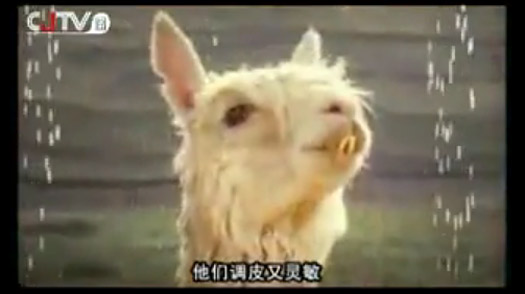
\includegraphics[width=3.7894in,height=2.1224in]{figures/chap2/chapitre2-img14.jpg}
    }
    \subfloat[Un caract\`ere chinois compos\'e sp\'ecialement par les internautes pour signifier cet animal mythique]{ 
        
\includegraphics[width=2.0559in,height=2.0559in]{figures/chap2/chapitre2-img15.jpg}
    }
    \caption[\textit{Caonima}: un animal mythique du web chinois]{\textit{Caonima}: un animal mythique du web chinois, d{\textquoteright}apr\`es le \textit{Grass-Mud Horse Lexicon Classics}publi\'e par \textit{China Digital Times }(2013)}
    \label{fig:caonima}

\end{figure}

Luttant contres les crabes de rivi\`ere, le \textit{caonima }symbolise la lutte contre la censure pour un Internet libre. Apparu pour la premi\`ere fois dans une vid\'eo virale\footnote{ \textit{Song of the Grass-Mud Horse (Cao Ni Ma), }Youtube \ \url{https://www.youtube.com/watch?v=wKx1aenJK08}, consult\'e le 28 F\'evrier 22:08\par }, le \textit{caonima} est un animal de la famille des cam\'elid\'es (l{\textquoteright}alpaga) courant fi\`erement dans les pr\'es sur une petite musique de dessin anim\'e aux paroles enti\`erement r\'e\'ecrites pour l{\textquoteright}occasion. Litt\'eralement {\textquotedblleft}cheval d{\textquoteright}herbe et de boue{\textquotedblright}, le mot {\textquotedblleft}caonima{\textquotedblright} [FF08?][8349?][6CE5?][9A6C?][FF09?]cache en fait un double sens puisque son homophone ([64CD?][4F60?][5988?]) est une grossi\`ere interjection \`a l{\textquoteright}intention des g\'enitrices des censeurs de P\'ekin. Devenu aujourd{\textquoteright}hui une v\'eritable ic\^one anti-censure, il n{\textquoteright}est pas rare de le croiser sur un tee-shirt ou accroch\'e \`a un sac dans de nombreux endroits improbables en Chine. Comme le note tr\`es justement An Xiao Mina : \textit{{\textquotedblleft}les m\`emes sont les graffitis du web censur\'e{\textquotedblright}} \cite{Mina2012}. Malgr\'e le z\`ele des pouvoirs publics \`a les effacer le plus rapidement possible, ils t\'emoignent de l{\textquoteright}existence de r\'ealit\'es occult\'ees qui se manifestent souvent de mani\`ere d\'erisoire, grotesque et improbable, mais sont \'enonc\'ees malgr\'e tout. 

\item[Publicit\'e et marketing viral]
\hfill \\
La popularit\'e des services de r\'eseaux sociaux a entra\^in\'e de nombreuses marques \`a se concentrer sur ce nouveau m\'edia pour mener leurs campagnes de publicit\'e et de promotion. Les utilisateurs chinois sont tr\`es fortement engag\'es dans la cr\'eation de nouveaux contenus avec 76\% des
utilisateurs chinois cr\'eant davantage de contenus qu{\textquoteright}ils n{\textquoteright}en lisent, contre seulement 20\% en France \cite{Forrester2012}. Ainsi, de nombreuses marques cherchent \`a concevoir des interactions en ligne utilisant les m\`emes comme v\'ehicule de messages commerciaux afin de
mettre \`a contribution les internautes dans la diffusion de leur marque. Une des strat\'egies marketing les plus r\'epandues consiste \`a cr\'eer un \textit{hashtag} amusant afin d{\textquoteright}inciter les internautes \`a s{\textquoteright}en saisir, le partager et cr\'eer de nouveaux
contenus. La marque de pr\'eservatifs \textit{Durex} a notamment connu un large
succ\`es avec le hashtag \textit{\#BienEtreNocturne} (en Chinois \#[591C?][798F?][5229?]) sur Sina Weibo. Dr\^ole et un peu os\'e, cette campagne a g\'en\'er\'e un fort engagement des internautes, contribuant largement \`a la propagation du profil utilisateur et du nom de la marque \cite{Shi2011}. En r\'ecup\'erant les donn\'ees des utilisateurs impliqu\'es dans la diffusion, la marque peut \'egalement proc\'eder \`a un travail statistique d{\textquoteright}analyse pour mieux conna\^itre les utilisateurs int\'eress\'es par ses produits.Ce type d{\textquoteright}information s{\textquoteright}av\`ere pr\'ecieuse dans un march\'e chinois en mouvement o\`u il existe un fort besoin pour des \'etudes de march\'e pr\'ecises aupr\`es de segments de populations actifs en ligne (adolescents, jeunes, classe moyenne \'emergente...) \cite{Bergstrom2012}. Malgr\'e le paysage morcel\'e des services de r\'eseaux sociaux chinois, les utilisateurs chinois semblent davantage enclins \`a suivre et interagir avec les marques que leurs homologues am\'ericains notamment\footnote{ D{\textquoteright}apr\`es Ken Hong, Sina Weibo General Marketing Manager  \url{http://adage.com/article/global-news/questions-sina-weibo-s-ken-hong-china/239508/,} consult\'e le 19 F\'evrier 2014 \`a 12:45}. 



\item[Marketing politique, soutien, p\'etitions]
\hfill \\
L{\textquoteright}industrie n{\textquoteright}est pas seule \`a s{\textquoteright}\^etre empar\'ee des r\'eseaux sociaux et les grandes entit\'es politiques ont \'egalement saisi \`a bras le corps ce nouveau m\'edia. Les plus brillants exemples sont sans doute les campagne men\'ees par Barack Obama pour la pr\'esidence des Etats-Unis. L{\textquoteright}importance capitale des r\'eseaux sociaux a plac\'e la strat\'egie de diffusion virale en haut de la pile des pr\'eoccupations pour l{\textquoteright}organisation de ces deux campagnes \'el\'ectorales \cite{Miller2008} avec notamment l{\textquoteright}utilisation de nombreux m\`emes pour f\'ed\'erer les votants. Lors de l{\textquoteright}\'etape de campagne aupr\`es des \'electeurs de l{\textquoteright}Ohio, un \'etat d\'ecisif de la course pr\'esidentielle, l{\textquoteright}\'equipe d{\textquoteright}Obama a notamment fait usage d{\textquoteright}un des fameux LOCats pur mobiliser son \'electorat. 


\begin{figure}
    \centering
    
\includegraphics[width=4.1669in,height=4.178in]{figures/chap2/chapitre2-img16.png}
    \caption[Lolcat utilisé lors la campagne d'Obama]{ 
        LOLCat utilis\'e durant la campagne d{\textquoteright}Obama en Ohio - d{\textquoteright}apr\`es \textit{Obama Campaign Deploys Cat Meme to Get Out the Vote in Ohio sur }Politicker, consult\'e le 28 f\'evrier 2008 \`a 11h41 GMT+1
    } 
    \label{fig:obama-cat}
\end{figure}

En Chine \'egalement, les r\'eseaux sociaux sont tr\`es utilis\'es pour la diffusion d{\textquoteright}id\'ees lors de campagnes politiques. Les groupes nationalistes soutenus par le gouvernement se saisissent r\'eguli\`erement de l{\textquoteright}actualit\'e pour rebondir et rassembler les foules \cite{Wu2007}. L\`a encore, les m\`emes jouent un r\^ole important dans l{\textquoteright}appropriation des discussions au travers de la r\'e-\'enonciation de sujets controvers\'es en des termes diff\'erents. Les tensions grandissantes entre les habitants du territoire de Hong Kong et ceux venus de la Chine int\'erieure ont \'et\'e notamment le sujet d{\textquoteright}une discussion int\'eressante par m\`emes interpos\'es. Les visites \`a Hong Kong sont tr\`es r\'egul\'ees pour les citoyens venus de Chine int\'erieure mais le flux massif de touristes n{\textquoteright}a n\'eanmoins cess\'e de cro\^itre depuis plusieurs ann\'ees avec l{\textquoteright}augmentation des quotas et l{\textquoteright}acc\`es aux cong\'es dans les grandes villes de la RPC. De nombreux chinois se rendent donc \`a Hong Kong pour voyager mais \'egalement profiter de la d\'etaxe des produits de consommation et des services publics de bien meilleure qualit\'e. La qualit\'e des h\^opitaux de la ville et l{\textquoteright}application du droit du sol dans la loi hongkongaise am\`enent de nombreuses jeunes m\`eres venues de Chine \`a traverser la fronti\`ere pour venir accoucher \`a HK. Cette pratique tr\`es controvers\'ee donne \`a l{\textquoteright}enfant le passeport hongkongais et se monnaie \`a prix d{\textquoteright}or, rendant l{\textquoteright}acc\`es aux hopitaux de plus en plus cher et attisant la col\`ere des habitants de HK. En septembre 2012, une p\'etition lanc\'ee \`a Hongkong a cherch\'e \`a recueillir des votes pour interdire l{\textquoteright}acc\`es aux h\^opitaux aux chinois venus de RPC. Un tract publi\'e pour cette campagne a largement circul\'e sur le web chinois ; on pouvait y lire :\textit{ {\textquotedblleft}Habitants de Hong Kong, nous avons assez souffert ! (...) Ne nous laissons pas envahir par la vermine venue de Chine int\'erieure.{\textquotedblright}}  

\begin{figure}
    \centering
    \subfloat[Le tract original] {
        
\includegraphics[width=3.3224in,height=2.4335in]{figures/chap2/chapitre2-img17.jpg}
    }
    \subfloat[Exemples de tracts r\'ealis\'es par les internautes en r\'eponse \`a la campagne]{
        % 
\includegraphics[width=1.4449in,height=2.178in]{figures/chap2/chapitre2-img18.jpg}
        
\includegraphics[width=1.4894in,height=2.1894in]{figures/chap2/chapitre2-img19.jpg}
        
\includegraphics[width=1.2894in,height=2.2224in]{figures/chap2/chapitre2-img20.jpg}
        % 
\includegraphics[width=1.3669in,height=2.2114in]{figures/chap2/chapitre2-img21.jpg}
    }
    \caption[Détournement de tracts hongkongais anti-chinois]{Détournement de tracts hongkongais anti-chinois,d{\textquoteright}apr\`es \textit{The Civic Beat, }\url{http://reader.thecivicbeat.com/2012/03/locusts-and-pandas-and-bears-??-o-mai/} consult\'e le 1er Mars 2014 \`a 22h58}
    \label{fig:hk-tract}
\end{figure}

Les internautes chinois choqu\'es mais arm\'es d{\textquoteright}un humour toujours tr\`es cinglant ont donc entam\'e une contre-campagne en proposant des versions modifi\'ees et r\'e\'ecrites du dit tract. R\'eactions \'epidermiques, propos nationalistes sommaires, mais aussi critique du tourisme de masse, d\'enonciation de la corruption et de la mauvaise qualit\'e des soins hospitaliers en Chine et nombreuses blagues absurdes, les adaptations et r\'eponses singeant le tract d{\textquoteright}origine ont montr\'e un panel d{\textquoteright}arguments et de r\'eactions qui a permis de crever l{\textquoteright}abc\'es et d{\textquoteright}ouvrir un d\'ebat national sur ce probl\`eme \'epineux r\'ev\'elateur des griefs actuels des habitants de HK envers ceux de la RPC.  


\item[Fan clubs, adoration]
\hfill \\
Comme tout mass media, les r\'eseaux sociaux poss\`edent une \'enorme quantit\'e de contenus consacr\'es aux stars, \`a leurs vies, leurs coups durs et leurs derniers films et chansons. D\'eveloppant des strat\'egies d{\textquoteright}envergure sur les m\'edias chinois, de nombreuses stars internationales ont fait leur arriv\'ee sur Sina Weibo comme notamment Brad Pitt ou Kobe Bryant. N\'eanmoins, leur influence reste incomparable \`a celles des stars originaires de Chine, de Taiwan et de Hong Kong ou bien encore de Cor\'ee du Sud, principal producteur de pop culture en Asie \cite{Martel2010}. Une des stars les plus pl\'ebiscit\'ee dans les r\'eseaux sociaux est pourtant une \'etrang\`ere puisqu{\textquoteright}il s{\textquoteright}agit de la japonaise Sola Aoi, ex-actrice de film pornographique devenu une des 10 personnes les plus suivies sur Sina Weibo avec pr\`es de 15 millions de followers\footnote{ D{\textquoteright}apr\`es Sina Weibo \url{http://www.weibo.com/1739928273/yBJYNt7Ol,} consult\'e le 1 Mars 2017 \`a 23h11}. Personnalit\'e m\'ediatique publique, la star a depuis plusieurs ann\'ees utilis\'e les r\'eseaux sociaux pour nouer contact avec le public chinois qui semble bien la conna\^itre, malgr\'e l{\textquoteright}interdiction de la pornographie en Chine. Aujourd{\textquoteright}hui retrait\'ee du monde du X \`a 30 ans, Sola Aoi utilise sa popularit\'e pour d\'efendre une paix durable entre la Chine et le Japon. Alors que les tensions politiques exacerb\'ees entre la Chine et le Japon ont men\'e \`a des rixes et des maltraitances envers les ressortissants dans les deux pays, elle a notamment contribu\'e \`a cr\'eer un appel \`a la non-violence sous forme de m\`eme \ qui a \'et\'e extr\^emement diffus\'e.  

\begin{figure}
    
\includegraphics[width=6.0114in,height=4.0114in]{figures/chap2/chapitre2-img22.jpg}
    \caption[La star du X japonaise Sola Aoi sur Sina Weibo]{Un message disant\textit{ {\textquotedblleft}Les peuples de la Chine et du Japon sont des amis{\textquotedblright} }post\'e par la star Sola Aoi}
    \label{fig:pornstar-weibo}
\end{figure}

Ainsi, les fan clubs et les stars elles-m\^emes jouent un r\^ole important dans la cr\'eation et la diffusion des m\`emes, occupant une large place dans le paysage m\'ediatique et notamment celui des r\'eseaux sociaux. 


\item[Hoax, spam]
\hfill \\
Un des plus c\'el\`ebres exemples dans ce domaine sont les emails dits
de {\textquotedblleft}fraude 4-1-9{\textquotedblright} cherchant \`a
extorquer de l{\textquoteright}argent au destinataire. Le num\'ero 419
correspond au num\'ero de l{\textquoteright}article interdisant la
pratique de l{\textquoteright}escroquerie en ligne dans le code p\'enal
nig\'erian. En effet, la forme la plus connue de cette arnaque est
celle du {\textquotedblleft}prince nig\'erian{\textquotedblright}
demandant un num\'ero de compte bancaire pour y transf\'erer rapidement
des fonds : 

\begin{figure}
    \begin{quote}
        I am Stella Amah 19 years of age the only daughter of late Mr Boni Amah whom was killed by the rebels that attacked our country cote d'Ivoire west Africa and took over our town (BOUAKE). I ran to Abidjan the economical capital of cote d'ivoire from were I am contacting you. Before the death of my father he told me that he has a sum of US\$9,000,000(Nine million united states dollars) kept in a private security company here in cote d'ivoire in my name as the next of kin... 
    \end{quote}
    \caption[Extrait d'un spam du type \textit{Nigerian Scam}]{
        Extrait d{\textquoteright}un {\textquotedblleft}Nigerian Scam{\textquotedblright}, d{\textquoteright}apr\`es \url{http://www.hoax-slayer.com/stella-amah-scam.shtml,} consult\'e le 2 Mars 2014 \`a 18h50
    }
    \label{fig:nigerian-scam}
\end{figure}

Adapt\'es sous de multiples formes, ce type de messages existent \'egalement sous les r\'eseaux sociaux sous la forme de \textit{bots}, comptes tenus par des robots postant des messages promotionnels. 

\end{description}

Au regard des diff\'erents exemples donn\'ees ici, nous voyons qu{\textquoteright}il est difficile de classer les m\`emes selon des cat\'egories pr\'ecises et qu{\textquoteright}en bien des endroits ces cat\'egories se recoupent : les stars font de la politique alors que les politiques font dans le comique. Ainsi, il ne s{\textquoteright}agit pas de dresser des cat\'egories rigides mais de disposer d{\textquoteright}une classification flexible pour pouvoir analyser les \'el\'ements discursifs pr\'esents dans les m\`emes Internet. La suite de cette \'etude interrogera plus pr\'ecis\'ement la constitution de ces formes de discursivit\'es dans leurs multiples~empiriquement observables par l{\textquoteright}analyse de donn\'ees issues de \textit{Sina Weibo}: structure du r\'eseau social, contenu des m\`emes, forme multim\'edia, \'el\'ements de contexte du message, etc. Nous allons donc maintenant pr\'esenter les m\'ethodes d{\textquoteright}extraction, de traitement et d{\textquoteright}analyse de donn\'ees en d\'etaillant la m\'ethodologie que nous avons retenue pour cette \'etude.